\documentclass[thesis]{subfiles}

\begin{document}
\chapter{Conditional Networks for Large Scale Visual Object Recognition}
\label{firstyear}

\subsection{Imagenet Large Scale Visual Recognition Challenge (ILSVRC)}
We validate the use of conditional networks for image classification on the ILSVRC dataset~\cite{ILSVRC2015}, a large dataset consisting of 1.2M training images for 1000 classes, and 50,000 validation images. The ILSVRC dataset has been of particular focus since the results of Krizhevsky et al.~\cite{Krizhevsky2012imanet} with the \emph{SuperVision} network, now commonly referred to as \emph{AlexNet}.

AlexNet uses two filter groups throughout most of the layers of the model in order to split computation across two GPUs. The authors observed that the filters on each GPU appeared to specialize to learn fundamentally different features regardless of initialization~\cite{Krizhevsky2012imanet}. This interesting observation has mostly been ignored in subsequent networks where GPU memory has increased enought that such a split of the network is not required, but the original observation is a fundamental motivation of our work.

We based our experiments on the VGG network~\cite{Simonyan2014verydeep} on which the current state-of-the-art models are also based~\cite{He2015delving}. Specifically, we focus on the VGG11 model as it is deep (11 layers) and relatively memory efficient (trains with Caffe on a single Nvidia K40 GPU). It notably does not have any filter grouping, as found in AlexNet, or low-dimensional embeddings, as found in network-in-network. It therefore suffers from and explosion in the number of filters required at each layer, and represents the ideal network on which to demonstrate the efficiency savings brought about by these simple modifications.

\subsection{Global max-pooling to reduce model size}
We found that global {\em max}-pooling, like 
{\em average}-pooling (as used in~\cite{Lin2013NiN,Szegedy2014going}), after the last convolutional layer is effective in reducing model parameters while maintaining, if not improving, accuracy. In VGG11 the input to the first fully connected layer (\ie \texttt{fc7}) consists of a tensor of size 
This suggests that preserving spatial information after the convolutional layers may not be as important as previously thought. 
We trained a new network (`VGG11-GMP') with such pooling, and achieved lower top-5 error than the baseline VGG11 
network (13.3\% \vs 13.8\%), with a decrease in the number of parameters of over 72\% (see Fig.~\ref{fig:VggPerLayerCost}).

\subsection{Designing an efficient conditional architecture}
Starting from the already improveld, unrouted VGG11-GMP architecture, we designed the conditional network in Fig.~\ref{fig:Imagenet_CondNet}.
% figure 
\begin{figure}[t]
\centerline{
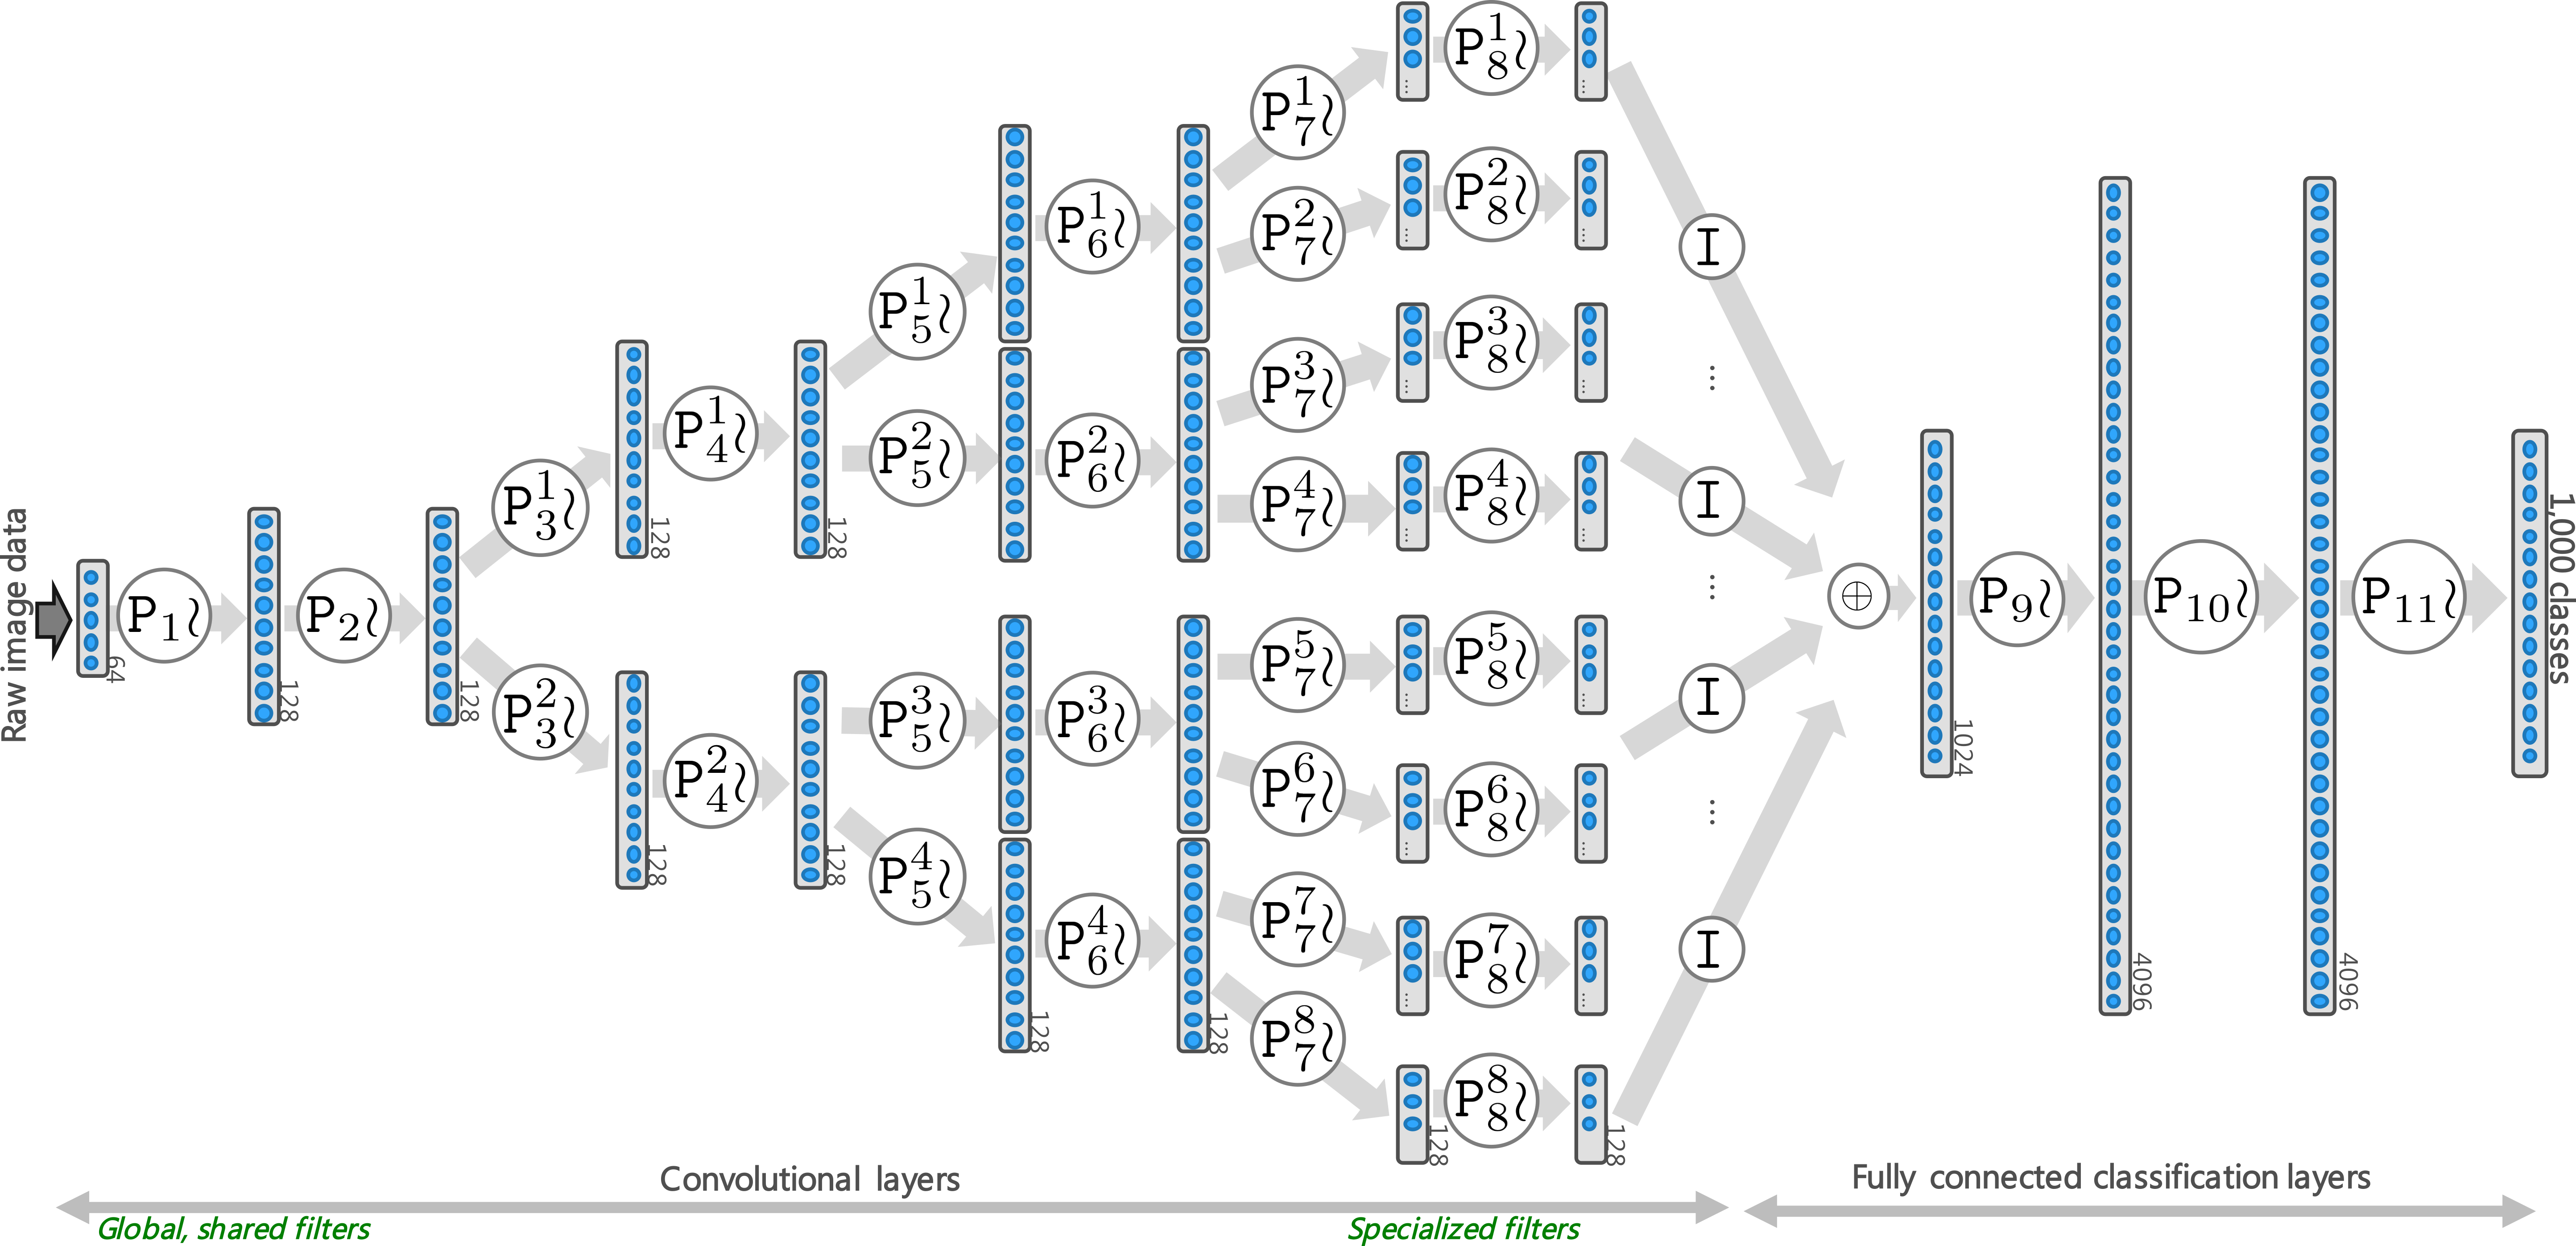
\includegraphics[width=1.1\linewidth]{resultsImagenet_conditionalNetwork}
}
   \caption{{\bf The conditional network used on the Imagenet experiments} employs implicit data routing in the 
   (expensive) convolutional layers to yield higher compute efficiency than the corresponding, unrouted DNNs.}
\label{fig:Imagenet_CondNet}
\end{figure}
%
Since most of the computational cost in VGG11-GMP is in the convolutional layers, our conditional variant 
introduces a DAG-like routed structure to split the filters in the convolutional section.
The assumption here is that each filter should only need to be applied to a small number of channels in the input feature map.

Data routing is implemented via `filter groups', as originally used in~\cite{Krizhevsky2012imanet}. 
Thus, at each level $\textrm{conv}\_n\_\{1,2\}, n=3\ldots 5$, the convolutional filters of VGG11-GMP are 
divided into $2^{(n-2)}$ groups. Each group depends only on the results of exactly 128 previous filters. 
The feature maps of the last convolutional layer are concatenated together, and globally max-pooled
 before the fully-connected layers, which remain the same as those in VGG11-GMP.

\subsection{Training}
We trained our conditional network with the same hyperparameters as in~\cite{Simonyan2014verydeep}, 
except for using the initialization strategy suggested of~\cite{He2015delving}, and a learning schedule of 
$\gamma_t = \gamma_0(1+\gamma_0\lambda t)^{-1}$, where $\gamma_0,\gamma_t$ and $\lambda$ 
are the initial learning rate, learning rate at iteration $t$, and weight decay respectively~\cite{Bottou2012sgdtricks}. 
When the validation accuracy of the network levelled out, the learning rate was further decreased by a factor of 10, twice. 
The conditional network took twice as many epochs to train than VGG11, however this equates to a comparable
 training time given its higher efficiency.

\subsection{Accuracy \vs efficiency results}
In order to compare different network architectures as fairly as possible, here we did not use any training
 augmentation aside from that supported by Caffe (mirroring/random crops). Similarly we report test-time 
 accuracy based only on centre-cropped images, without potentially expensive data oversampling. 
 This reduces the overall accuracy (w.r.t.\ to state of the art), but constitutes a fairer test bed for 
 teasing out the effects of different network architectures.
Applying the same oversampling to all networks produced a nearly identical accuracy improvement in 
all models, without changing their ranking.

%%% Figure ---------------


\begin{figure}[htbp!] 
\centering
\begin{subfigure}[b]{\textwidth}
   \centering
   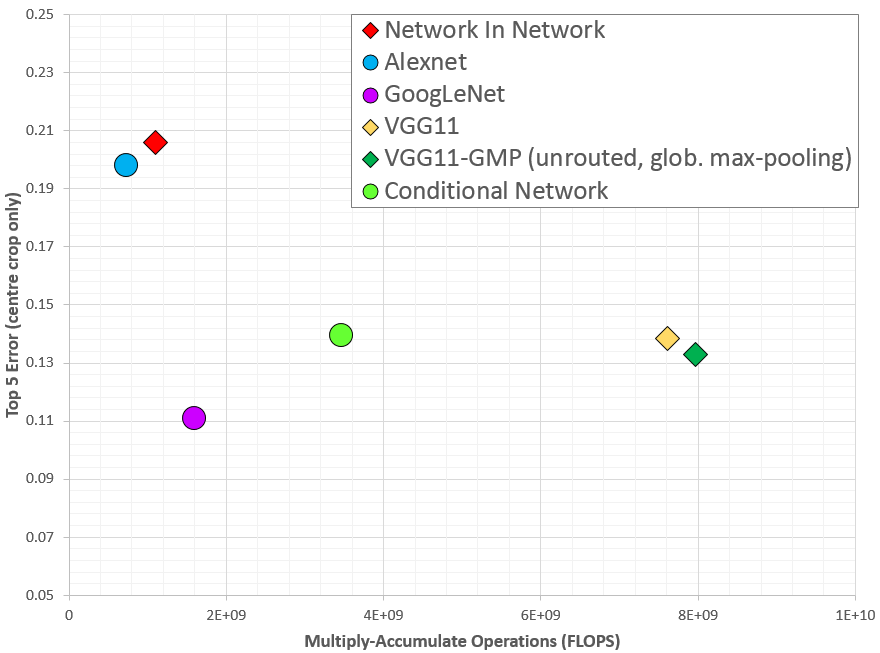
\includegraphics[width=0.9\textwidth]{resultsImagenet_AccVsEff}
   \caption{Top-5 ILSVRC validation error (centre crop) \vs compute for various network architectures.}
   \label{fig:resultsImagenet_AccVsEff}
\end{subfigure}
~
\begin{subfigure}[b]{\textwidth}
   \centering
   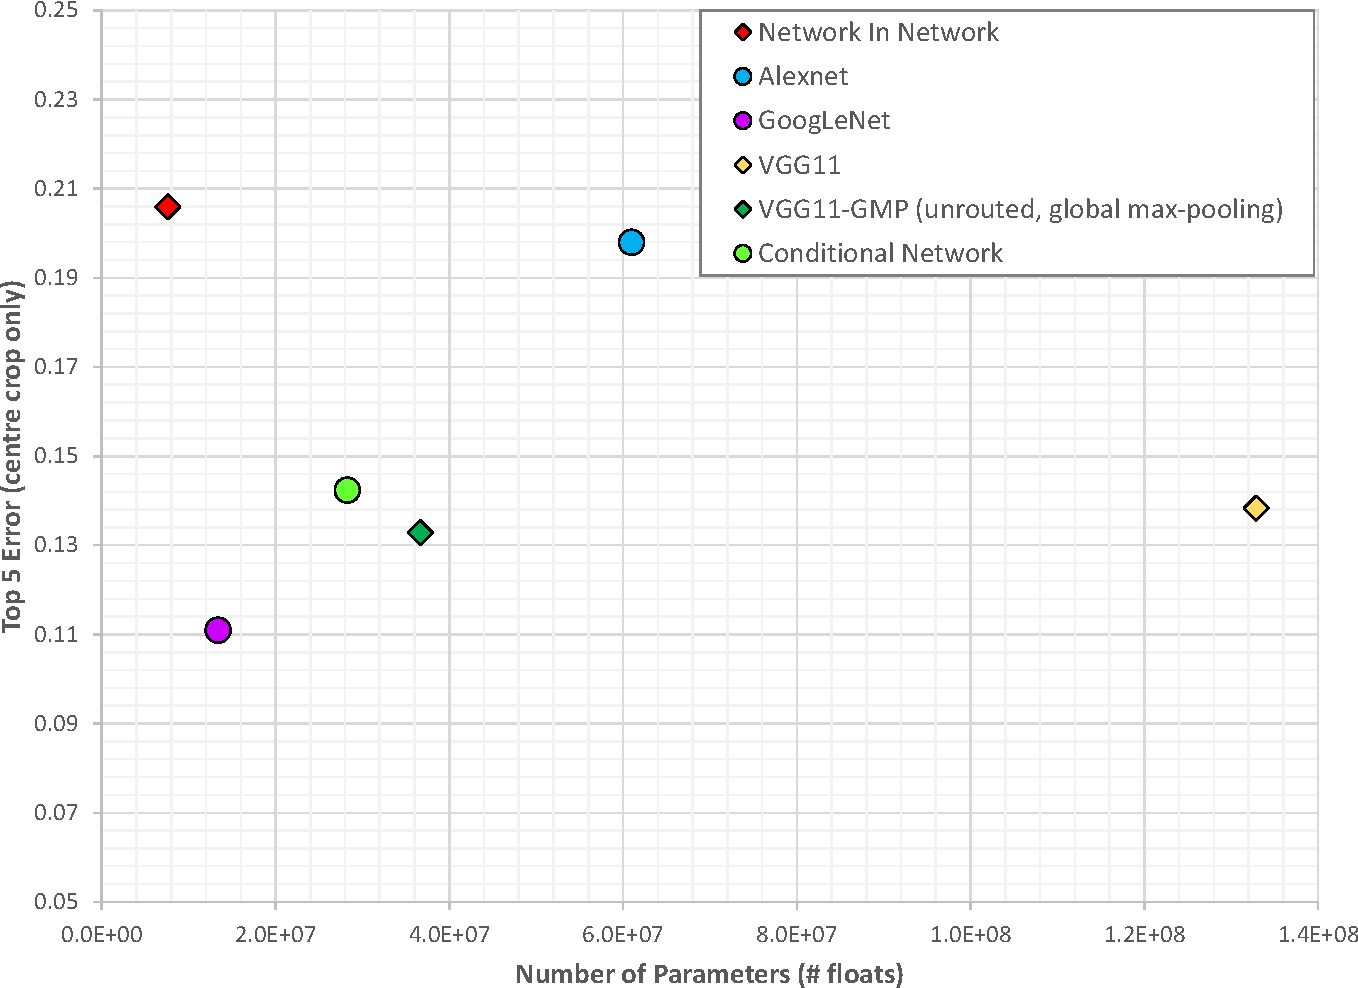
\includegraphics[width=0.9\textwidth]{resultsImagenet_AccVsSize}
   \caption{Top-5 ILSVRC validation error (centre crop) \vs model size for various architectures.}
   \label{fig:resultsImagenet_AccVsSize}
\end{subfigure}
\caption{Our VGG11-GMP (green diamond in \ref{fig:Imagenet_results} reduces model size significantly. Conditional networks (denoted with circles) yield points closest to the origin, corresponding to the best accuracy-efficiency trade-off. Best viewed on screen.}
\label{fig:Imagenet_results}
\end{figure}


Figure~\ref{fig:Imagenet_results} summarizes the results.
It shows top-5 error as a function of test-time 
cost\footnote{measured here as number of multiply-accumulate operations. We have observed this measure 
to correlate very well with CPU time.} and model size. 
The best network (closest to the origin) is GoogLeNet~\cite{Szegedy2014going} (in purple), it is very accurate and efficient. 
GoogLeNet and Alexnet~\cite{Krizhevsky2012imanet} (in light blue) are in fact instances of conditional networks 
(though they were not presented that way). In both networks much of the compute saving is obtained by routing
 subsets of features to different branches of the network.
In addition, GoogLeNet learns low-dimensional embeddings, has multiple intermediate training losses, and a very 
different training schedule. These differences, along with its deeper DAG structure, may explain its superior performance.

The conditional network of Fig.~\ref{fig:Imagenet_CondNet} 
corresponds to the green circle in Fig.~\ref{fig:Imagenet_results}.
It achieves a top-5, centre-crop error of
13.9\% compared to 13.8\% for the VGG11 network, while requiring less than half of the compute (45\%),
 and almost one-fifth (21\%) of the parameters.
Although it is the second closest to the origin (after GoogLeNet) we believe that better results can be achieved 
by using routes of different (learned) cardinality, as well as incorporating low-dimensional embedding and multiple-loss training. This is left for future work. 
Note that the most efficient model in~\cite{He2015delving} uses 1.9E+10 flops which is just outside the plot. 
More accurate versions of~\cite{He2015delving} are more expensive still.
Finally, Fig.~\ref{fig:VggPerLayerCost} shows efficiency improvements achieved by our conditional network, layer by layer.

%%% Figure ---------------
\begin{figure}[t]
\centerline{
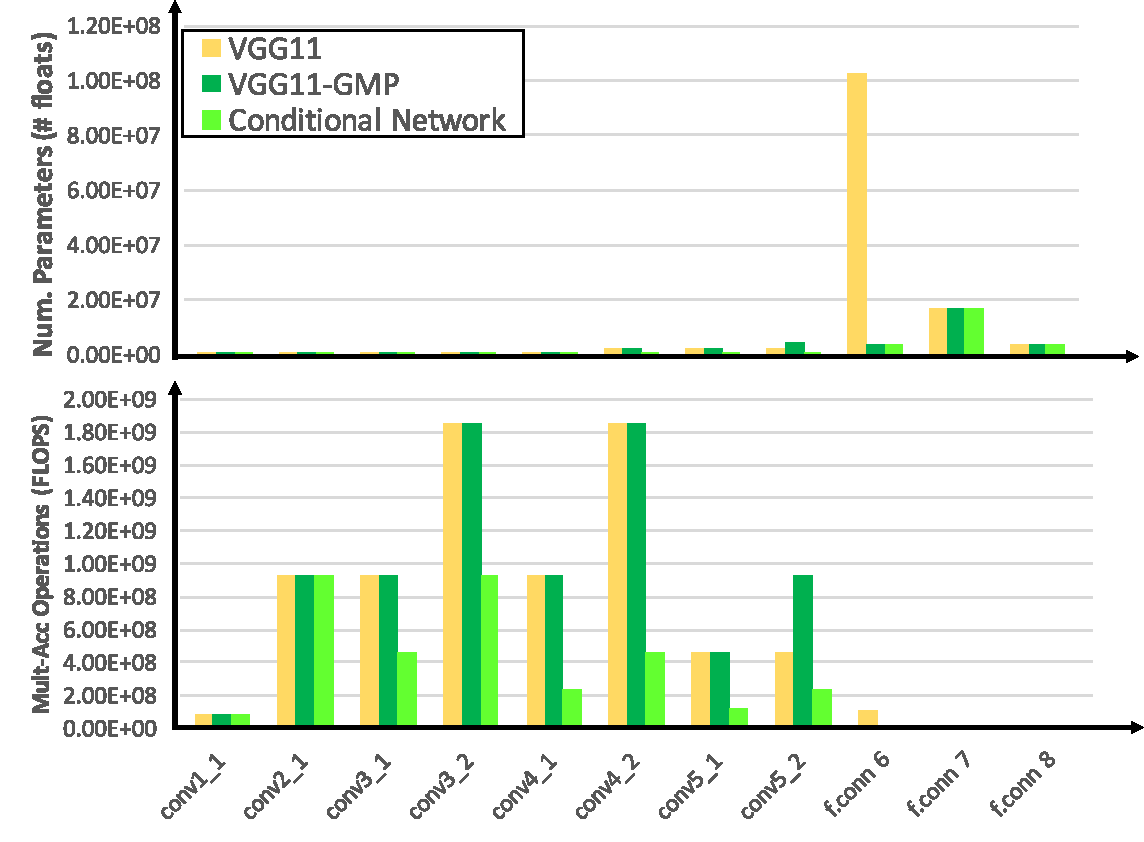
\includegraphics[width=\linewidth]{vgg11costs}
}
   \caption{{\bf Cost of VGG11-based networks per layer}. 
   Number of parameters and number of multiply-accumulate operations for all (convolutional and fully-connected) 
   layers of VGG11, VGG11-GMP, and our conditional network. Our two networks (dark and light green) 
   reduce both the memory use and the compute cost.}
\label{fig:VggPerLayerCost}
\end{figure}


% Removed to save space
%GoogLeNet divides filters within each ``inception'' module into 4 groups of various filter sizes, 
%giving the overall network a DAG-like structure. GoogLeNet's usage of low-dimensional embeddings within 
%these routes reduces compute and parameters of the network even further.


%The most efficient of the state of the art networks used for Imagenet classification, by a wide margin, is 
%GoogLeNet (see fig.~\ref{fig:Imagenet_results}). Network in Network and GoogLeNet pioneered the use of semi-dense 
%weight matrices in the form of learning dimensionality reductions, reducing the explosion of filters usually found in deep network architectures.

%Another unique feature of these two networks is global average pooling, where the spatial dimensions of the last convolutional 
%feature map are reduced to a single compact feature vector of length $f$, where $f$ is the number of filters in the layer. 
%This greatly reduces the parameters of the network by reducing the weights in the first fully-connected layer, which contains 
%the majority of weights in the network (see fig.~\ref{fig:VggPerLayerCost}), and is the single largest factor in the space efficiency of Network in Network and GoogLeNet.

%\begin{itemize}
%\item Our convtree has much more potential for distributed computation.
%\item Hyper-parameter optimization - we use the same hyper-parameters as VGG, but less regularization may be required with 20\% of the param.
%\item Our structure is much simpler than that of GoogLeNet and much less optimized.
%em We train each conditional network plotted in the graph from scratch while they build on top of already trained networks. 
%This is important for reproducibility of results. Very difficult to reproduce their results and to extend them to other datasets or domain. 
%We demonstrate our model on ImageNet AND CIFAR too.
%\item We can take existing networks (VGG/MSRA) and improve them by adding routing.
%\item They have such a complex and long structure that they need to train using intermediate losses with manually set weights.
%\end{itemize}

\section{CIFAR10}
Here we validate conditional networks for the classification of images in the CIFAR10 dataset~\cite{CIFAR10}. 
The dataset contains 60,000 images of 10 classes, typically divided into 50,000 training images and 10,000 test images. 
We take the state of the art Network in Network (NiN) model 
as a reference~\cite{Lin2013NiN}, and we build a conditional version of it to produce the architecture in Fig.~\ref{fig:Cifar_CondNet}. 
Then we go on to show its increased efficiency compared to the original NiN model.
%\acnote{there is another net which is 0.1\% better.}

% figure 
\begin{figure}[t]
\centerline{
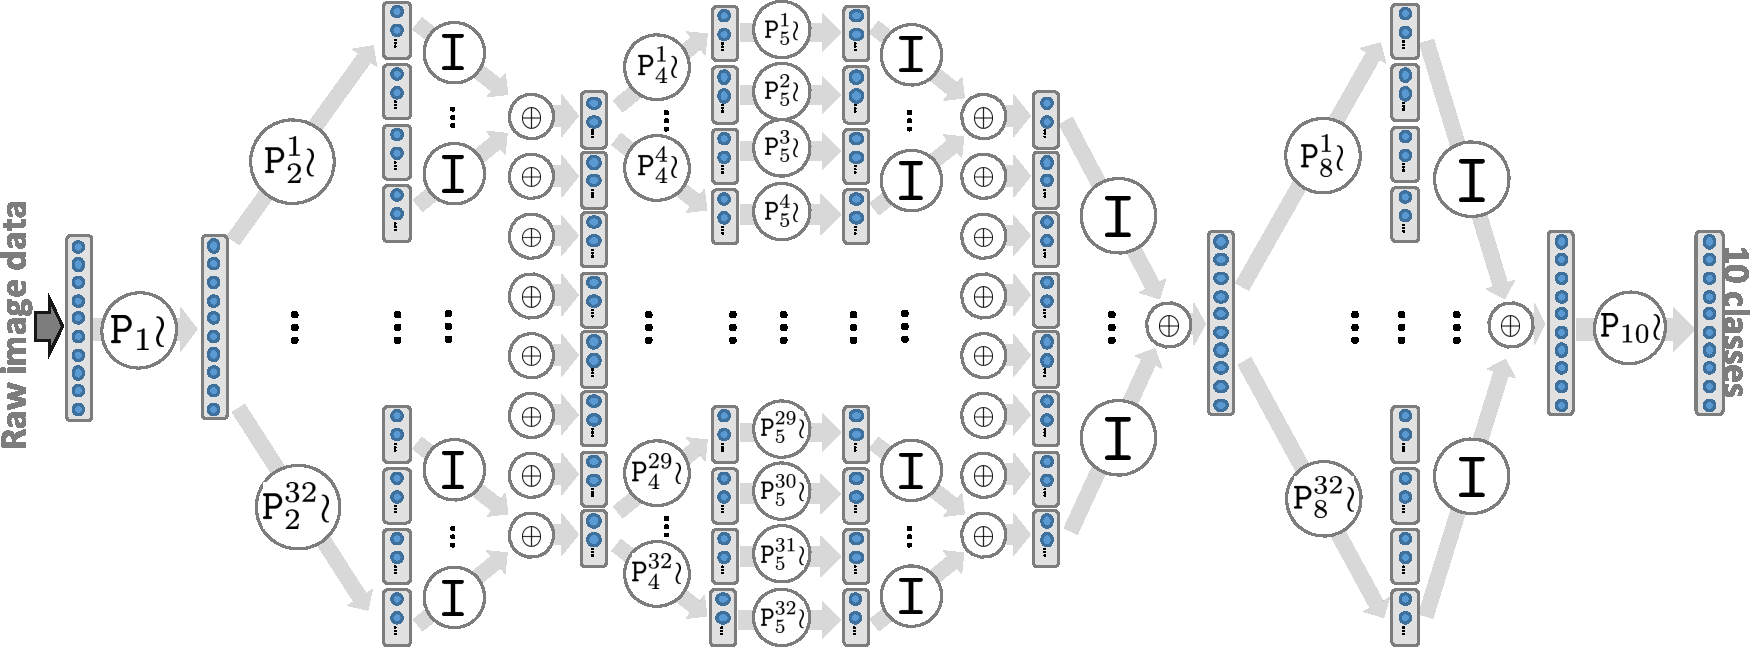
\includegraphics[width=1.1\linewidth]{resultsCifar_conditionalNetwork}
}
   \caption{{\bf Automatically learned conditional architecture for image classification in CIFAR.} Both structure and parameters of this conditional network have been learned automatically via Bayesian optimization.
Best viewed on screen.}
\label{fig:Cifar_CondNet}
\end{figure}

\subsection{Designing a family of conditional networks}
The NiN model has a large number (192) of initial image-level filters in the first convolutional layer (`conv1'), 
representing a sizable amount of the overall compute.\footnote{Most Imagenet networks typically use $64-96$ conv1 filters.}

We build a variant (`NiN-64') that prepends a layer of 64 filters to the NiN model.
While this variant is more complex than NiN, when routed (as described later) it allows us 
to split the larger layers into many routes and increase the efficiency.
In fact, for a convolutional layer with $N$ groups of filters, each filter operates on $1/N$ channels of the input feature map, thus yielding reduced test-time computation and learning filters with fewer channels. 
Additionally, training routed convolutional layers means that filters are exposed only to the training subset of data that flows through that route, thus allowing for a potentially higher degree of specialization.
By changing the number of routes at each level of the NiN-64 model (from conv2) we can 
generate a whole family of possible conditional architectures. 

\subsection{Learning the optimal network architecture}
In this experiment we have optimized the network structure {\em automatically}, 
by using Bayesian optimization~\cite{Snoek2012}, as available in WhetLab.\footnote{https://www.whetlab.com} 
This has allowed us to search the large joint space of parameters and structures in a principled way, 
and come up with multiple reasonable networks to be tested. 
%\acnote{we have not done this in Imagenet because too big.}

In the optimization we maximized the {\em size-normalized} accuracy $\alpha =\frac{\textrm{classification accuracy}}{\textrm{model size}}$ with respect to the parameters $R_l = 2^i, \left\{i\in \mathbb{N} : 0 \le i \le 5\right\}$, where $R_l$ is the number of nodes at layer $l$ in the conditional network. 
Fig.~\ref{fig:Cifar_CondNet} shows the architecture which maximizes $\alpha$ in CIFAR10. 
It is a DAG-structured conditional network with 10 layers.
To our knowledge this is the first attempt at learning automatically the architecture of a deep CNN for image classification.

\noindent{\bf Accuracy \vs efficiency results.}
For comparison, we also reduce the complexity of the unrouted NiN-64 network by learning a reduction in the number of per-layer filters. 
\ie we maximize $\alpha$ over $F_l = F_\textrm{orig}/2^i, \left\{i\in \mathbb{N} : 0 \le i \le 4\right\}$, where $F_\textrm{orig}$ is the number of filters in layer $l$ in NiN-64. 

All networks were trained with the same hyperparameters as~\cite{Lin2013NiN}, 
except for using the initialization strategy of~\cite{He2015delving}, 
and a learning schedule of $\gamma_t = \gamma_0(1+\gamma_0\lambda t)^{-1}$, where $\gamma_0,\gamma_t$ and $\lambda$ are the initial learning rate, learning rate at iteration $t$, and weight decay respectively~\cite{Bottou2012sgdtricks}. Training was run for a maximum of 400 epochs, or until the maximum validation accuracy had not changed in 10,000 iterations. 
We split the original CIFAR10 training set into 40,000 training images and 
10,000 validation images. 
The standard 10,000 held-out images are used for testing.


\begin{figure}[htbp!] 
\centering
\begin{subfigure}[b]{\textwidth}
   \centering
   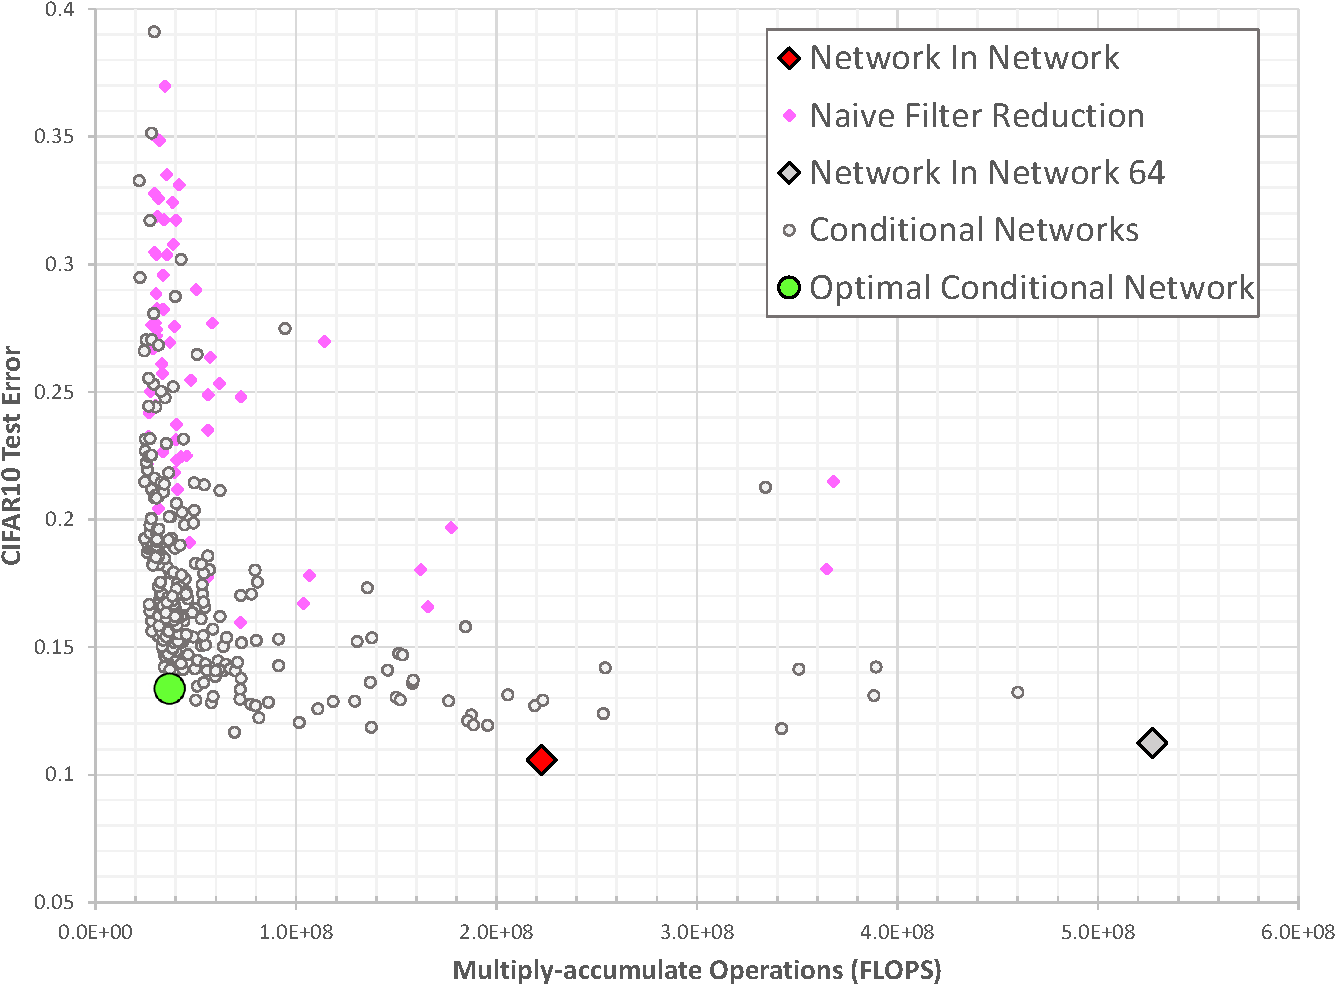
\includegraphics[width=0.9\textwidth]{resultsCifar_AccVsEff}
   \caption{Test error \vs test-time compute for various architectures used in the CIFAR experiments.}
   \label{fig:resultsCifar_AccVsEff}
\end{subfigure}
~
\begin{subfigure}[b]{\textwidth}
   \centering
   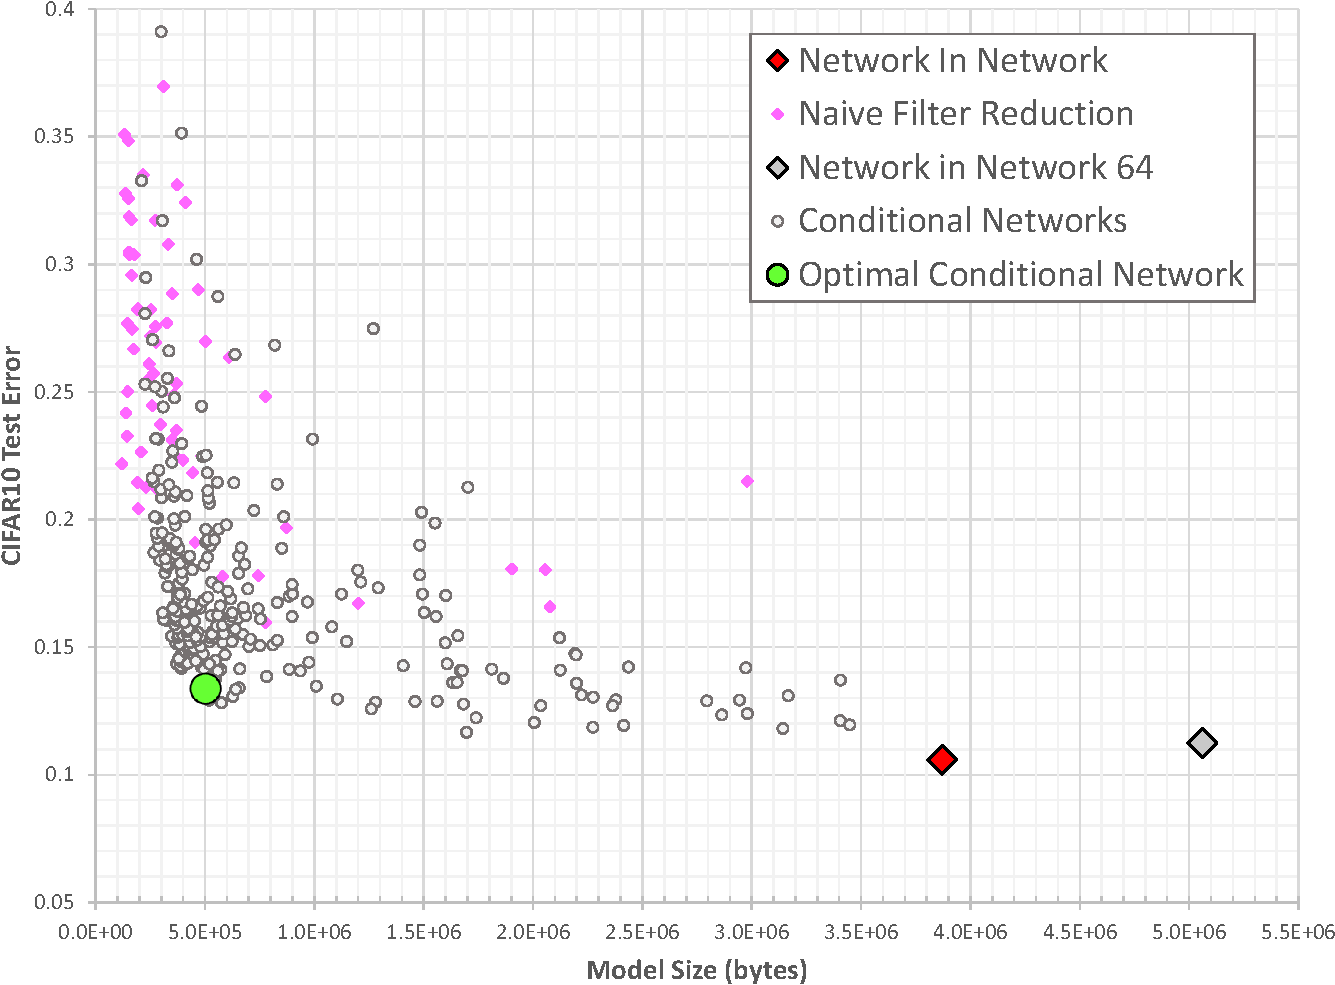
\includegraphics[width=0.9\textwidth]{resultsCifar_AccVsSize}
   \caption{Test error \vs model size.}
   \label{fig:resultsCifar_AccVsSize}
\end{subfigure}
\caption{{\bf Comparing network architectures on CIFAR10.} Conditional networks (denoted with circles) yield the points closest to the origin, corresponding to the best accuracy-efficiency trade-off. Our best conditional network is denoted with a green circle. See text.}
\label{fig:Cifar_results}
\end{figure}
%
Fig.~\ref{fig:Cifar_results} shows test errors with respect to test-time cost and model size for multiple networks.
Diamonds denote unrouted networks and circles denote conditional networks. 
The original NiN is shown in red, and our NiN-64 variant is shown as a grey diamond.
A sample of 300 models explored during the Bayesian optimization are shown as grey circles.
The green circle denotes the conditional network closest to the origin of the 
3D space $(test-error,test-cost,model-size)$.
Most of the conditional networks proposed by the Bayesian search procedure are distributed along a curve characterized by either high accuracy, or low model size, or both. 
Reducing the NiN model by filter reduction (pink diamonds in the figure) does not yield the same gains as data routing.
Despite NiN achieving the highest accuracy (it has been optimized for accuracy alone), the optimal conditional network is much closer to the origin of the 3D space, thus indicating much higher efficiency (in terms of memory and compute) for a small loss in accuracy.



%\acnote{Show results when using full training (50000). In the same plot. Or say something about this in one line.}

% Maybe remove the following?
%\acnote{Need to show results when training is optimized for accuracy only, without drop-out. To see if grouping provides any regularization.}

\end{document}